\documentclass[12pt,letterpaper]{report}
\usepackage{graphicx}
\usepackage[latin1]{inputenc}
\usepackage{amsmath}
\usepackage{amsfonts}
\usepackage{amssymb}
\usepackage[left=3.0cm,right=3.0cm,top=3.5cm,bottom=2.5cm]{geometry}
\author{Mihael Hategan}
\begin{document}
\section{Terminology (tasks, jobs, workers, etc)}

\begin{description}
	\item[Task] A task is a possibly long running thing at the cog kit level. There are three major types of tasks: execution, file transfer, and file ops. Execution tasks encapsulate everything that is needed to run a process (e.g. executable, arguments, env. vars, etc.). File transfer tasks should be self-explanatory. File ops are operations that can be done on a filesystem, such as file listing, directory creation, etc. Within swift user-level lingo, tasks are instances of apps.
	
	\item[Provider] A provider is a piece of code that can run tasks. Multiple provider implementations allow ``running'' tasks using various mechanisms (SSH, GRAM, GridFTP, HTTP, etc.). In some cases (coasters), a provider can delegate certain functions to other providers. For example, starting the coaster service is done by launching a (possibly remote) process. This is done using any of the existing execution providers.
	
	\item[Job] We decided to use the term ``job'' to signify a LRM job. However, in the general sense, job is any long running user code, and, while such jobs can be run through a LRM, it is not necessarily the case. Context can usually be used to tell what exactly is meant by ``job''.
	
	\item[Workers] (i.e. ``pilot jobs'' or ``glide-ins'') are those things that are started by coasters (or an equivalent mechanism) on compute nodes to handle user tasks.
\end{description}

\section{How Swift throttles foreach loops}
	Swift can in theory run all iterations of a foreach loop in parallel. This is sometimes unnecessary, since there is no point in queuing a large number of tasks out of which only a few can run due to a limited number of compute-cores being available. For this reason, Swift has the ability to limit the number of iterations that a foreach loop will have running in parallel. There is one setting for all foreach instances, so it must be used in conjunction with some source-level analysis. For example, to limit the number of user level-tasks in a script in which there are two nested foreach loops to a value $n$, one would have to limit the number of parallel foreach iterations to $\sqrt{n}$.

\label{s:tasks}
\section{How swift presents tasks to providers (ie, how they get batched)}

As soon as all dependencies of an app task are satisfied, the task switches to the "Selecting Site" state and attempts to get a site from the karajan task scheduler. As soon as the relevant throttles permit, a site is assigned to the app task, after which the app task is sent to one of the three staging implementations (swift-staging, provider-staging, wrapper-staging). From there on, things depend on this choice as follows:
	\begin{description}
		\item[swift-staging] In this mode, the following steps are taken:
			\begin{itemize}
				\item Initialize site shared directory if this is the first app task running on this site
				\item Create all directories needed by task input and output files in the site shared directory
				\item Stage in files in the site shared directory
				\item Run swiftwrap with relevant parameters
				\item Check result (by detecting whether swiftwrap produced a success file or an error file)
				\item Stage out files from the site shared directory if swiftwrap ran successfully
				\item Removing files from the site shared directory if disk space is needed (decided based on a user-specified maximum disk usage amount). This is a feature is not used much AFAIK.
			\end{itemize}
			
			All of these steps are done by queuing relevant cog-level tasks to the karajan scheduler, which will execute them according to the throttling/scheduling parameters.
			
			On the remote site, swiftwrap takes care of creating a local directory structure in the app task directory, copying or linking input files from the site shared directory to the app task directory and copying the output files to the 
			
		\item[provider-staging] This is a lot simpler, since all the directory creation and staging are delegated to the provider that runs the app task. Swift simply passes a list of stageins and a list of stageouts as a parameter to the cog task object and the execution provider does the actual work
		
		\item[wrapper-staging] This is somewhat similar to provider-staging, except the stageins and stageouts are passed to swiftwrap who then does the staging
	\end{description}

\section{Scheduling in the coaster provider}

	Is this separate from the box packing stuff?
	
	Tasks that get submitted to the coaster service get queued. A thread periodically re-calculates block requirements based on the queued tasks and constraints. It then starts or shuts down blocks accordingly. Tasks are then knapsacky sent to the idle workers. In other words, when a worker becomes idle, it will get the largest job that can fit in its remaining walltime. This strategy separates the slow process of calculating block requirements from the process that needs to be fast: dispatching tasks to workers.

\section{How coasters does its box-packing calculations}

This is essentially in the paper, but it goes along the following lines:

\begin{enumerate}
	\item Sort the queued tasks by walltime
	\item Figure out how many blocks to allocate by multiplying $slots - usedSlots$ with $allocationStepSize$. In other words, $newBlocks = ceil((slots - usedSlots) * allocationStepSize))$
	
	\item Divide the total size of the queued tasks among $newBlocks$. The basic idea is that there is some abstract notion of task size, and blocks have some abstract notion of capacity. If you have more than one block and you are trying to determine what capacity they should have, there is no unique way of doing that. You need to divide partition the total task size somehow. One way is to divide it equally among the new blocks and the other is to spread things out a bit. Two modes of spreading the taskss are provided: linear and exponential. A rough picture of this is provided in Figure \ref{f:spread}
	
	\begin{figure}[h]
		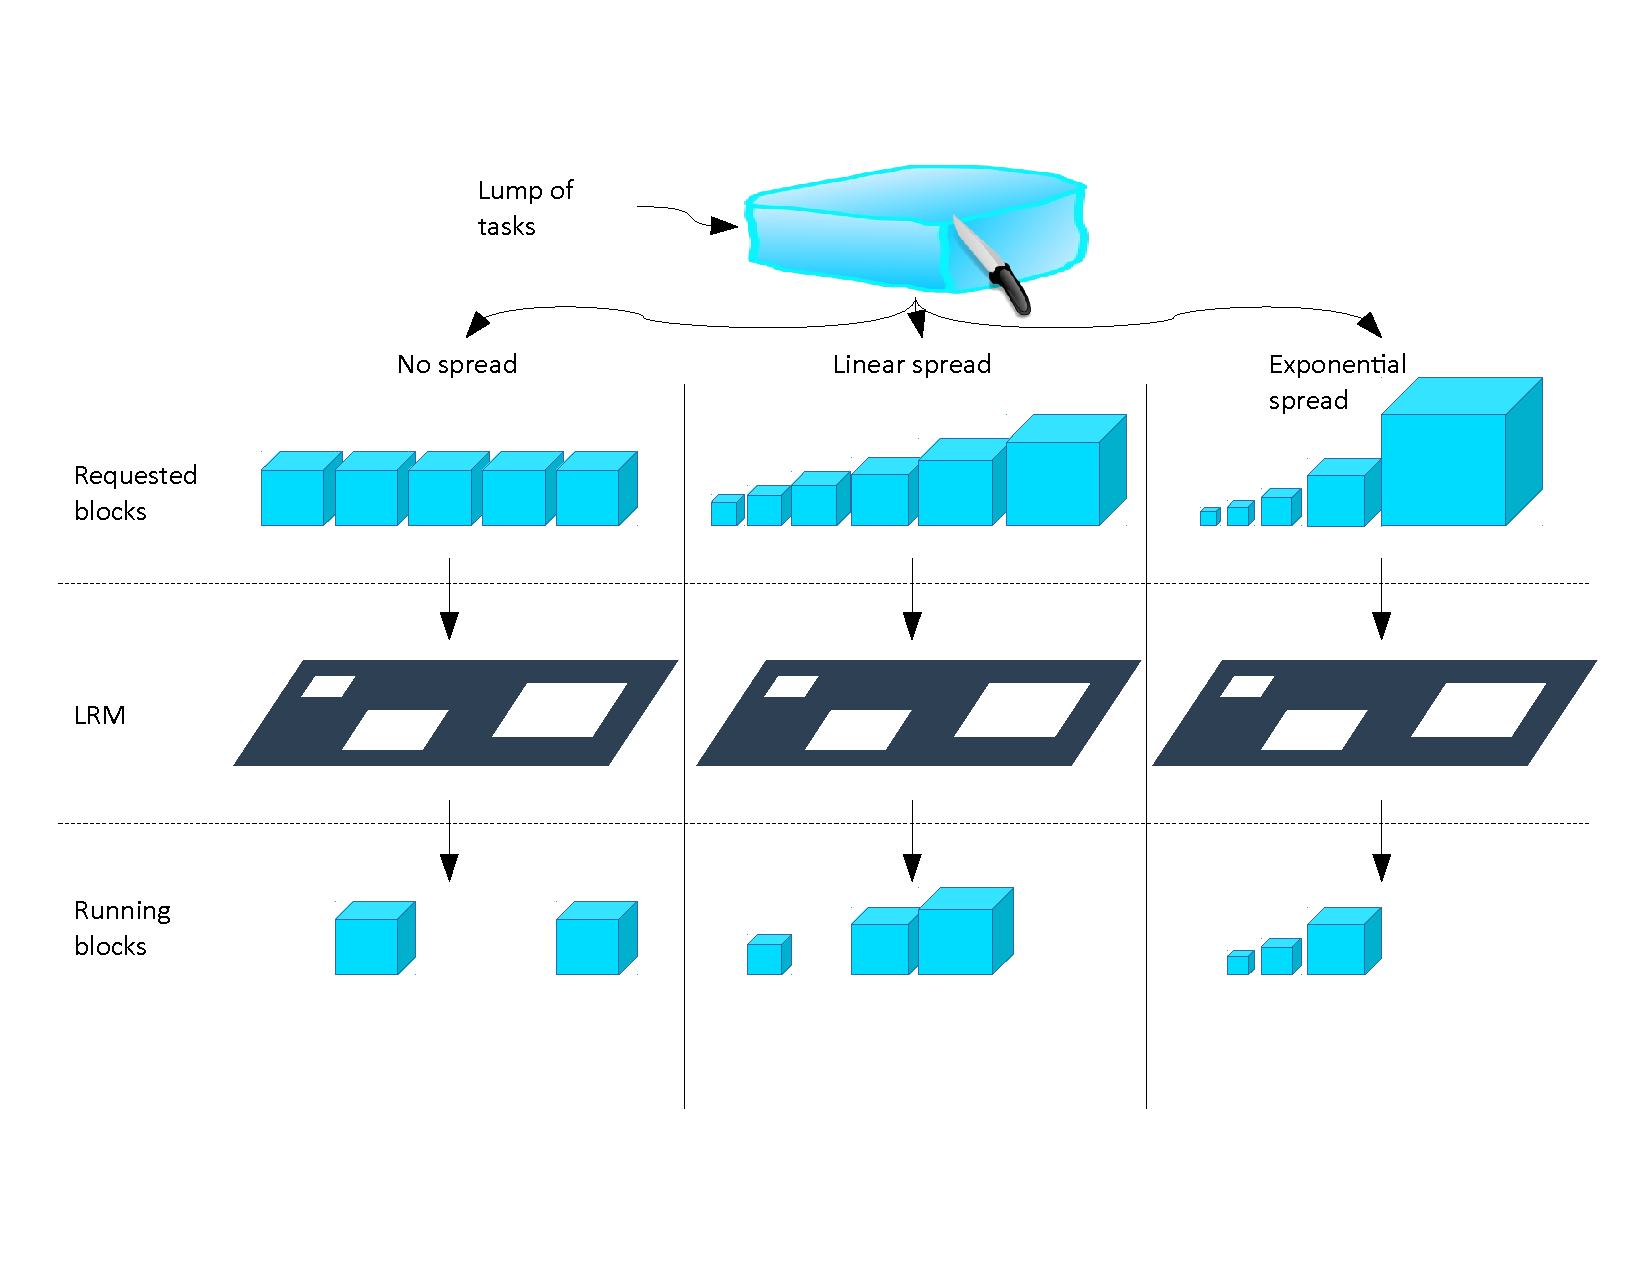
\includegraphics[scale=0.5]{spread.pdf}
		\caption{Spreading tasks into blocks}
		\label{f:spread}
	\end{figure}
	
	\item Once the general capacity of each block has been calculated, one needs to determine the exact shape of the block, since the capacity is a function of both walltime and number of cores (see Figure \ref{f:blockshape}). It goes like this:
		\begin{enumerate}
			\item Compute overallocated size based on the first task in the queue (i.e. how many re-uses of a block are wanted for taskss of this size)
			\item Cap to \texttt{maxtime} if needed
			\item Compute the number of cores by dividing the capacity of the block by the overallocated walltime and rounding based on granularity and \texttt{maxnodes}
		\end{enumerate}
		
		\begin{figure}[h]
			\center
			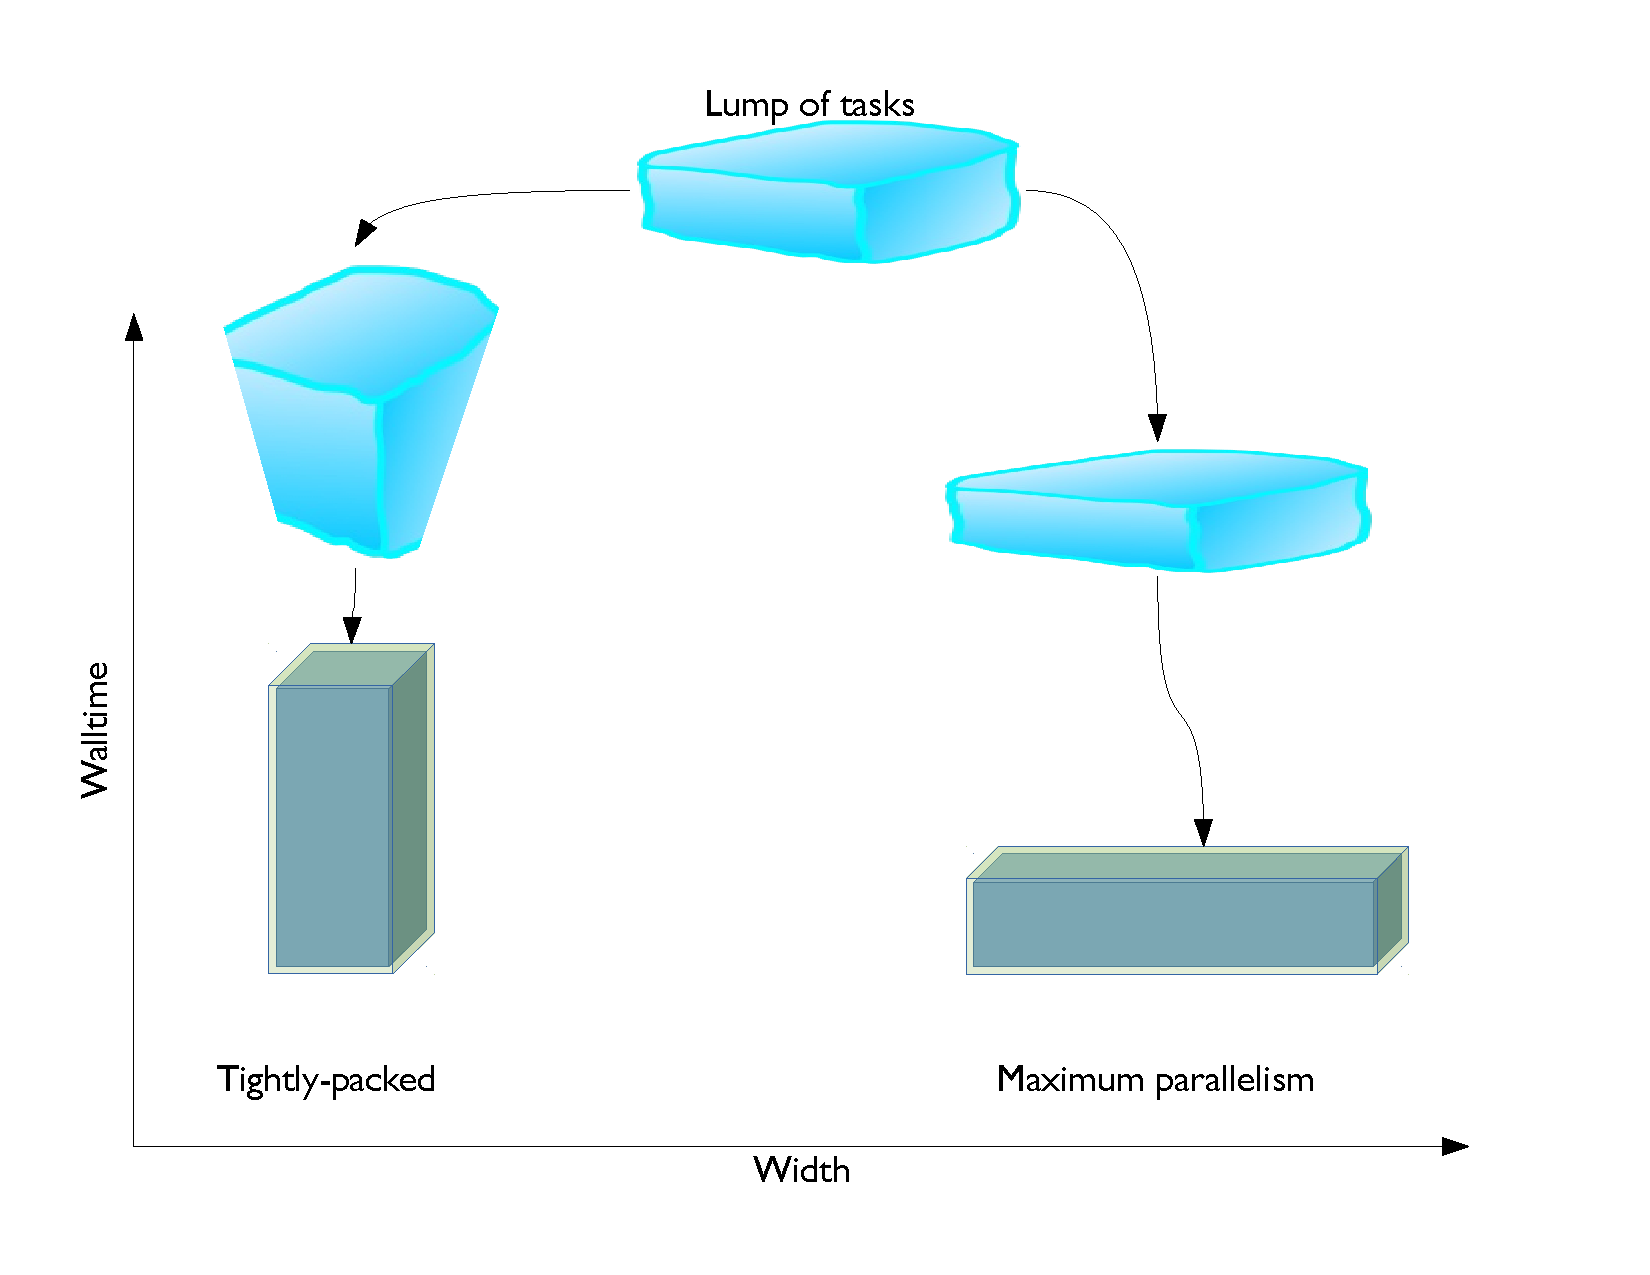
\includegraphics[scale=0.35]{blockshape.pdf}
			\caption{Block shape}
			\label{f:blockshape}
		\end{figure}
		
	\item ``Commit'' all tasks that can be fit to the newly created block (i.e. remove the tasks from the queue and put them in a ``ready-to-run'' pool)
	\item Start the block
\end{enumerate}

One thing to mention is that block capacity and job size are not some well defined concepts. They must, however, depend on walltime and width, since those are the only numbers available. There are two extremes:
\begin{enumerate}
	\item The size of a (single-core) task is its walltime. The capacity of a block is its walltime times its width (number of cores). This results in tight packing of tasks into blocks.
	\item The size of a task is its width (one for non-MPI jobs) and the size of a block is its width. This results in maximizing parallelism, but it likely produces temporary overestimates of block walltime. See Figure \ref{f:parallelism}
\end{enumerate}

The \texttt{parallelism} setting can be used to pick a smooth point somewhere in between the two extremes.

\begin{figure}[h]
	\center
	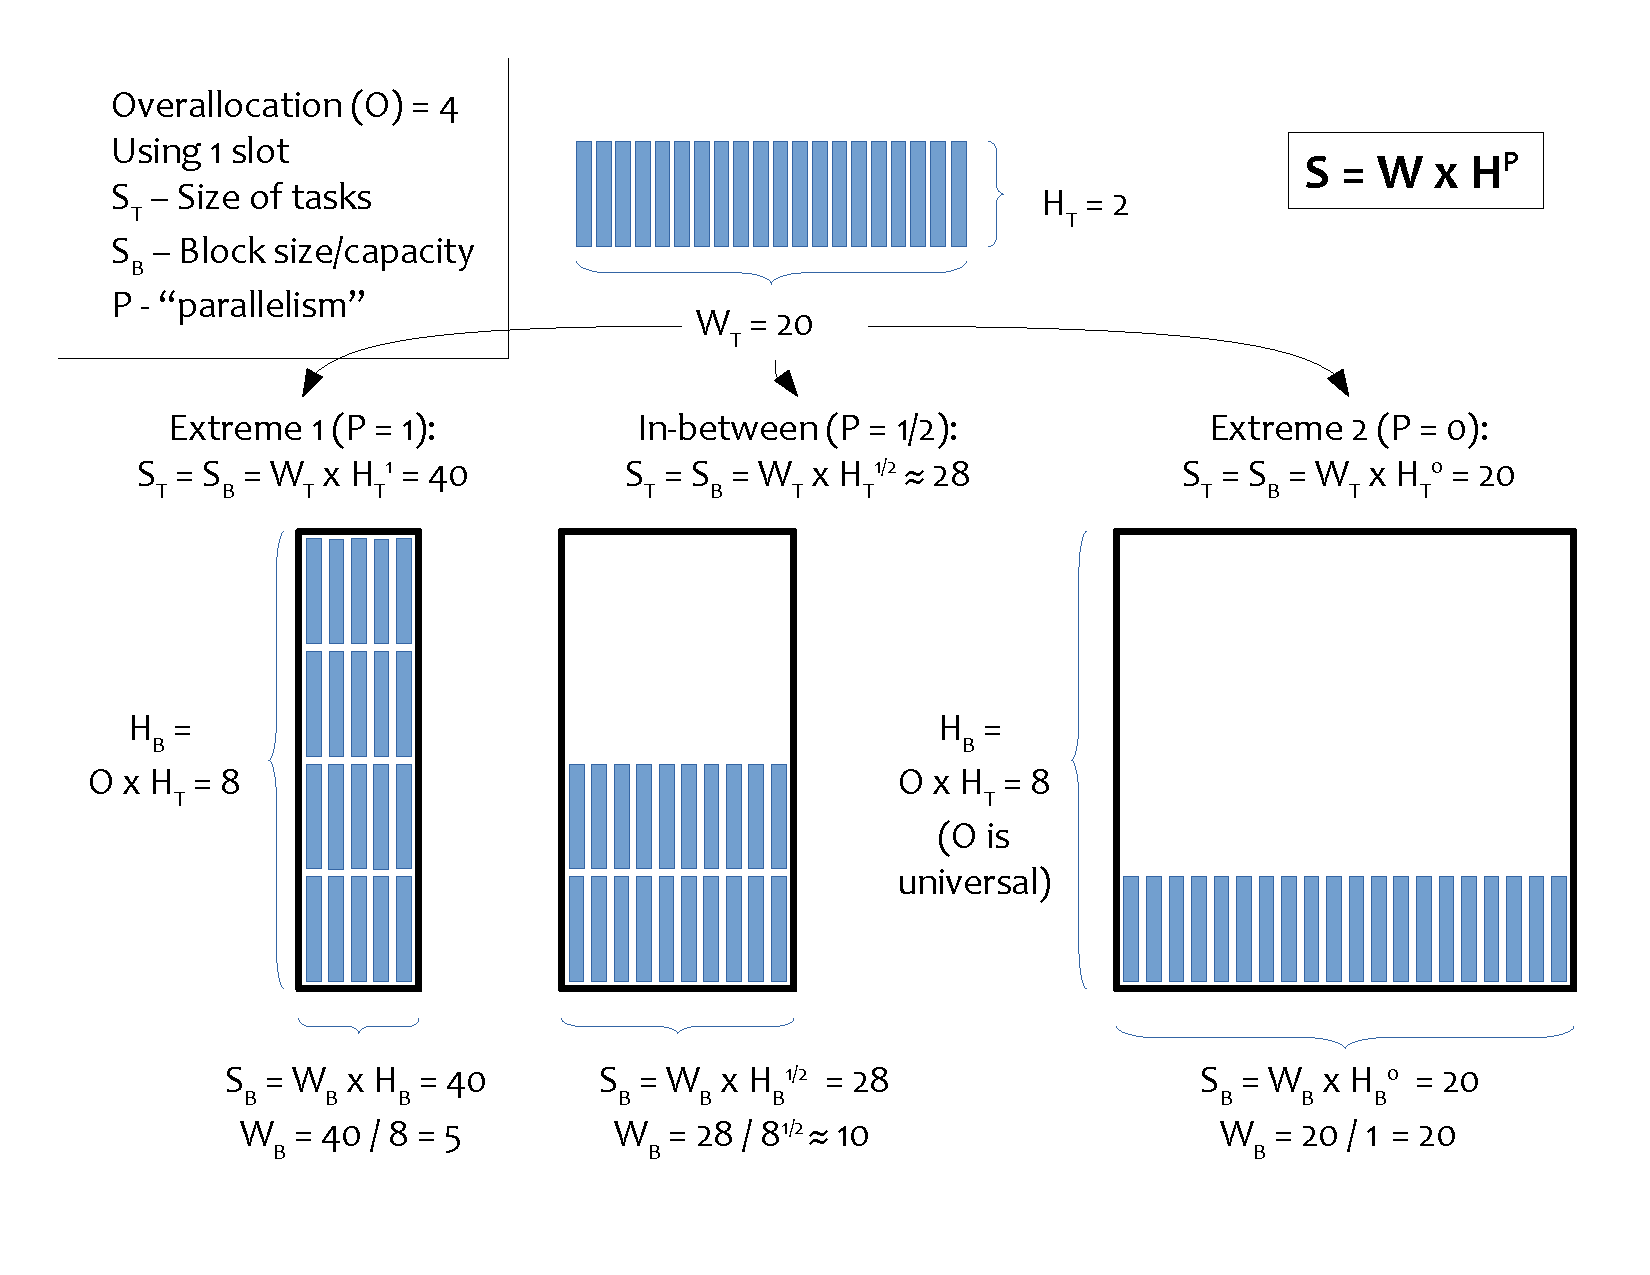
\includegraphics[scale=0.5]{parallelism.pdf}
	\caption{Parallelism}
	\label{f:parallelism}
\end{figure}

\section{Coaster worker linger time}

The removal of blocks works by sorting the blocks by their remaining useable time and trying to fit all remaining tasks in those blocks. Remaining blocks enter a ``suspended'' state if they have not seen any new tasks for a certain amount of time (i.e. they were idle for a while). Once suspended, a block gets shut down as soon as it finishes running its last task. The sorting is done in order to allow freeing as much of the schedule as possible. If one would try to fit remaining tasks into the largest block first, that block may very well be much larger than the capacity needed, so only a small portion of it might be used. See Figure \ref{f:linger}.

\begin{figure}[h]
	\center
	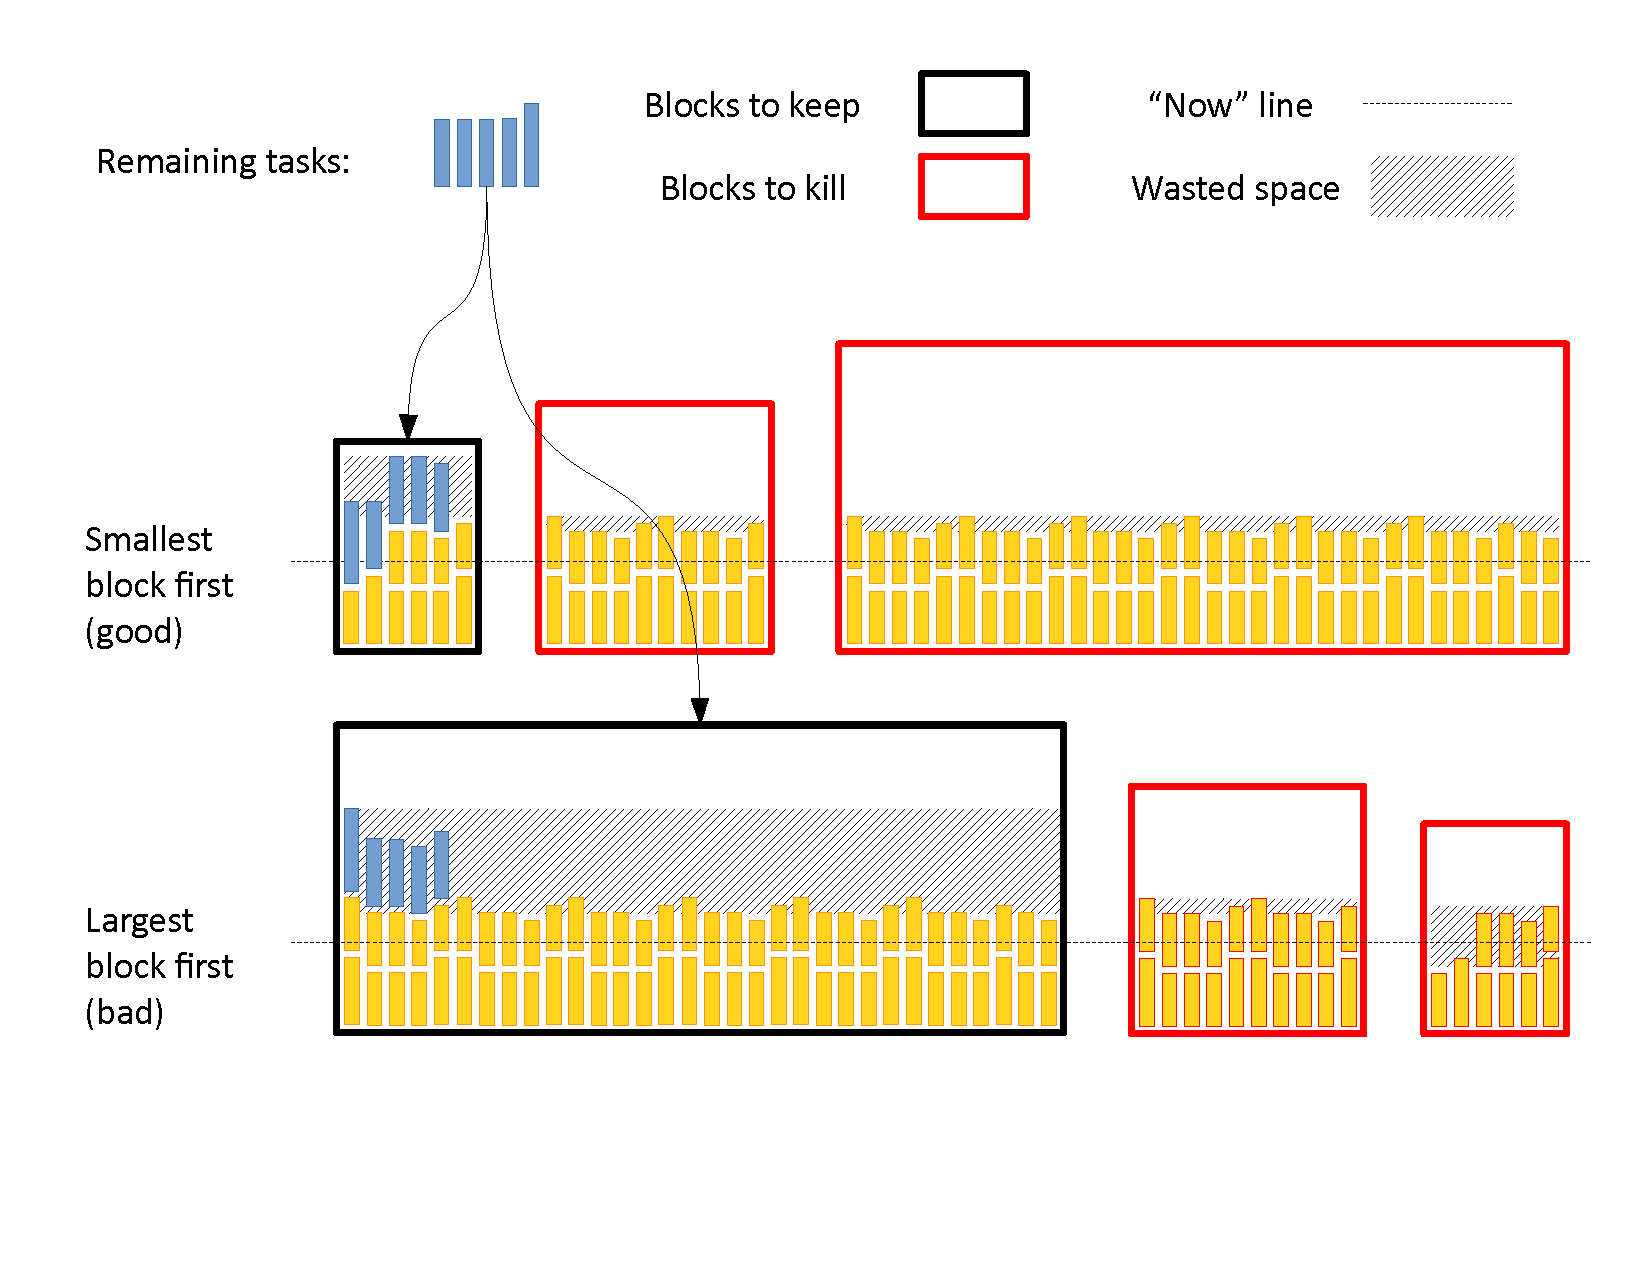
\includegraphics[scale=0.5]{linger.pdf}
	\caption{Block removal choices}
	\label{f:linger}
\end{figure}


\section{Handling of the per-site throttle logic}
...(and any of the older throttles that used to be specified in swift.properties - presumably 
these are still there)

There are two basic types of throttles: task throttles and task submission throttles. 

Task throttles are enforced for the entire duration of the task. For example, given a throttle of 10 and a bunch of \texttt{sleep 10} tasks, at most 10 \texttt{sleep 10} processes will be running at a time.

Task submission throttles are enforced only during the \texttt{provider.submit(task)} call. The origins of this date back to GRAM. When submitting a job, a GRAM client would connect to a GRAM server, send the job data and then disconnect. Part of this process included SSL/GSI session negotiation and possibly delegation (which involved generating a key pair and signing its certificate). This was a heavy CPU-bound process that limited the average submission rate of jobs to maybe 2 per second on the typical hardware of the time. Parallelizing this was only beneficial up to the number of cores the client had available (and detrimental soon after) since you can't make a CPU-bound process faster than the CPU power you have. There is little downside to having this throttle set to a not-so-high number: providers that can submit jobs fast will quickly free the slots for new jobs to be submitted; providers that are slow in submitting jobs are probably CPU-bound an therefore unlikely to benefit from massive multiplexing of a few CPU cores.

Other than that, there are throttles for each individual task type. Additionally, throttles can either be global (for the entire client) or per-site. All these can be combined to give you \texttt{[host](job|fileTransfers|fileOperations)[Submit]throttle}. Ever since file transfers and file operations were switched to use cached/persistent connections (e.g. by keeping GridFTP connections up for some time), the submit throttles for transfers/fileOps became slightly useless, so I am not sure to what extent they are exposed in swift.conf.

\section{How Swift handles site selection and dynamic site biasing}

The gist of it is, well, credit scores. Two factors enter the credit score calculations: current load (utilization if you will) and past task completion history. In essence, the more tasks running on a site, the lower its score AND the more tasks completed successfully by a site, the higher the score AND the more tasks failed by a site, the lower the score. The score for each site is capped at some value. When the scheduler needs to decide where to run a job based on the available sites, it makes a probabilistic decision based on the scores of the sites. In other words, the probability of a job going to a site $s$ is $p = \dfrac{Score_s}{\sum_{i \in all-sites} Score_i}$. If a site score becomes lower than a certain value, it is banned from running any new tasks for a certain amount of time that depends on exactly how low the score is. This is roughly an exponential back-off.

\section{When data transfers are done (especially where this relates to site 
selection decisions)}

See Section \ref{s:tasks}

\section{When site dirs and task dirs (sandboxes) are created and cleaned up}

This depends on the staging mode as follows:

\begin{description}
	\item[swift-staging] 
		\begin{itemize}
			\item Site dirs are created before the first app task is run and cleaned when the run completes. The cleaning is done by submitting a \texttt{rm -rf sitedir} job. Swift submits the \texttt{rm} job with the \texttt{batch} flag set, so in most cases this will result in the run ending after the job is queued, but not before it completes.
			\item Task dirs are created and removed by swiftwrap
		\end{itemize}
	
	\item[provider-staging]
		\begin{itemize}
			\item There is no site dir
			\item The task dir might be created by the provider if there are any stage-ins (it automatically creates necessary directories for staged-in files), or by swiftwrap. The task dir is removed by the provider through task cleanup directives.
		\end{itemize}
	
	\item[wrapper-staging]
		\begin{itemize}
			\item There is no site dir
			\item swiftwrap creates and removes the task dir
		\end{itemize}
\end{description}

\section{How data transfer / management throttles affect this, and scheduling}

What does ``this'' refer to here?

With swift staging, since all operations are directed by swift, site directory creation is governed by file ops rules (i.e. fileOperationsThrottle). The removal, since it is done using a job, this would be affected by the \texttt{jobSubmitThrottle}. The \texttt{hostJobSubmitThrottle} won't matter since there is at most one \texttt{rm} job per site/host.

With provider and wrapper staging, there are no explicit throttles. Coasters do some memory management when it comes to file transfers since it limits the total amount of buffers used to convey data from disk to the network. That can be seen as a throttle of sorts.

\end{document}